\documentclass[11pt, a4paper]{article}
\usepackage[greek,english]{babel}
\usepackage[linesnumbered,ruled]{algorithm2e}
\usepackage{graphicx}
\usepackage[titletoc,title]{appendix}
\graphicspath{{./Figures/}}
\setcounter{tocdepth}{3}
\linespread{1}
\title{\huge\textbf{Clever Support for 3D Printing}\\~\\\large CMPT464/764 ~\\Geometric Modeling in Computer Graphics~\\Course Project}
\author{~\\~\\Yiji Wang\\301286922 \and ~\\~\\Jack Anderson\\301126642 }
\date{~\\~\\Supervised by~\\Prof. Richard(Hao) Zhang~\\~\\~\\~\\April 15, 2016}
\begin{document}
    \maketitle
    \thispagestyle{empty}
    ~\\~\\~\\
    \begin{abstract}
        ~\\In this project, we implemented a tree-like support structure for 3D printing based on Fused Deposition Modeling(FDM) from paper: Clever Support: Efficient Support Structure Generation for Digital Fabrication.$\cite{paper}$~\\The overhangs pf the model need to be supported by connecting them with either part of the object or the printing layer using support material for 3D printing. Since the support material will be removed after printing, reducing the amount of the support can lead to less printing time and material waste. We implemented a novel, geometry-based approach that can minimize the support material used and provide sufficient support for the object.
    \end{abstract}
    \newpage
    \linespread{2}
    \tableofcontents
    \thispagestyle{empty}
	\newpage
	\linespread{1}
	\section{Introduction}
	\setcounter{page}{1}
	3D printing is becoming more and more popular in recent years with the general public due to lower prices and greater accessibility of 3D printers. There is less material wasted and greater model complexity when compared with traditional manufacturing methods like forging and CNC. In this project, we focus on the Fused Deposition Modeling(FDM) printers because they are the most common, inexpensive and widely used.
	
	~\\The printing process starts from the printing layer and then successively printing each slice until the printer reaches the top. Every 3D printer has a critical angle which means the maximum angle of a structure the printer can print without support. Therefore to print the overhangs, support is needed. Unlike other printers using cheap material, FDM printers use main printing material for support structures. Since the main printing material is used for supports, the support material usually costs a lot, nearly half of the model and the support material will be manually removed and cannot be reused. Most 3D printing softwares along with the printer generate the support structures by adding columns connecting the overhangs with printing layer or the model, leading to the amount of support material being unnecessarily large. 3D printing will become more accessible to the public with much less printing waste and printing time if less support structure is needed to be printed.

	~\\In this project, we implemented a novel, geometry-based solution to minimize the amount of support material. The input model was first oriented to a good position to reduce the area of overhanging parts. Then the sample points were detected from the overhanging parts and the support structure were iteratively built starting with these points. Instead of constructing a column for each overhang point, we built a tree-like structure to minimize the amount of support.

	~\\We compared the result of our implementation with the result provided by the author, the performace is close to the results from the Clever Support paper $\cite{paper}$ with models having less features while not so good with models having a lot more details. The average difference is around 20\%.
	\newpage
	\section{Implementation}
	\begin{figure}[!ht]
  		\centering
      	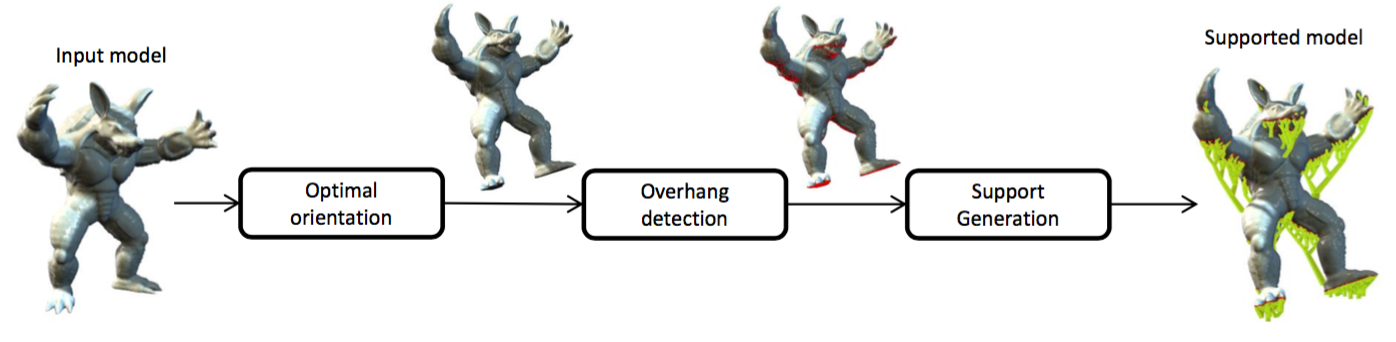
\includegraphics[width=1.0\textwidth]{Figure_1.png}
  	\caption{\textit{The pipeline of the system. The input is a 3D model represented by a manifold mesh. Further inputs are: the number of random rotation angles, critical angle of the printer, the sampling distance and the thickness of the support structure.}}
	\end{figure}
	

	\subsection{Optimal Orietation}
	In the first step, the model was rotated to a good orientation with less overhanging parts. Instead of using brute force method, which may give the best result but will lead to much more computation time, we used a simpler and faster heuristics provided in the paper.$\cite{overhang}$ First the number of random rotation angles $K$ is given as input, we generated $K$ different rotation angles. For each angle, we detected the overhanging points. To accelerate the process, we rotated the printing direction to find the best result among the candidates and applied rotation to the model for the best angle.$\cite{rotation}$ 

	\subsection{Overhang Detection}
	The support structure is generated from overhanging points. To obtain the overhanging points, first overhanging parts need to be deteceted and then uniform sampling will be applied to the overhang faces/edges.
	\subsubsection{Overhang parts detection}
	There are three types of overhangs need to be detected. Figure 2 shows two of them.
	\begin{itemize}
	\item Point Overhang
	~\\A point will be detected as point overhang if it's locally or globally lower than (in printing direction) all its neighbors.
	\item Face Overhang
	~\\Face overhang is a triangular face. Faces will be detected as overhang faces if the angle between the face and the printing direction $Y_p$ is greater than the critical angle. As shown in Figure 2, face 1 doesn't need support because $\alpha_1 < \alpha_c$ while face 2 does for $\alpha_2 < \alpha_c$.
	\item Edge Overhang
	~\\Edge detection is not used in our implementation because face and point overhang detection will cover the majority of cases where an edge needs to be supported.
	\end{itemize}
	\begin{figure}[!ht]
  		\centering
      	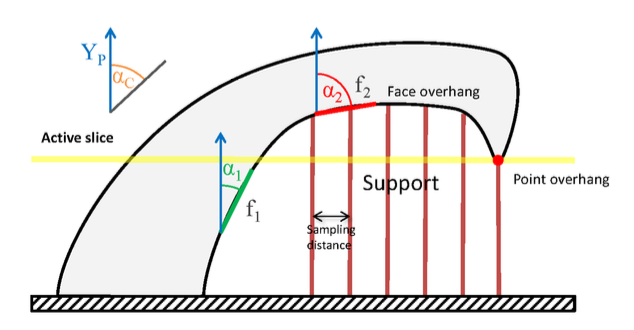
\includegraphics[width=0.8\textwidth]{Figure_2.png}
  	\caption{\textit{Point overhang and face overhang example. Point overhang is any point which is lower than all of its neighbours relative to the printing plane. Face overhang is any face whose angle with the printing direction is larger than the critical angle.}}
	\end{figure}
	\subsubsection{Uniform sampling}
	The support structure is generated from overhanging points. To obtain the overhang points, we did uniform sampling for the overhang faces and edges. The sampling distance is one of the inputs provided. Here we applied software scan-line rasterization algorithm.$\cite{sampling}$
	
	~\\Algorithm is below:
	\begin{enumerate}
	\item Find the minimum and maximum value of $z$ coordinate and $x$ coordinate of the model respectively, denote them as $x_{min}, x_{max}, z_{min}, z_{max}$.
	\item Apply scanning face starting from $z=z_{min}$, ending with $z=z_{max}$, moving along its normal $(0,0,1)$. If face f has intersection with $z=m$, apply the same scanning method for x coordinate moving along its normal $(1,0,0)$. 
	\item Get overhang points P from intersections of $z=m$, $x=n$ and face f
	\item Check whether the interseciton point is in the triangle using method from $\cite{pint}$
	\item Repeat step 2, 3 and 4 for every faces of the model
	\end{enumerate}
	\begin{figure}[!ht]
  		\centering
      	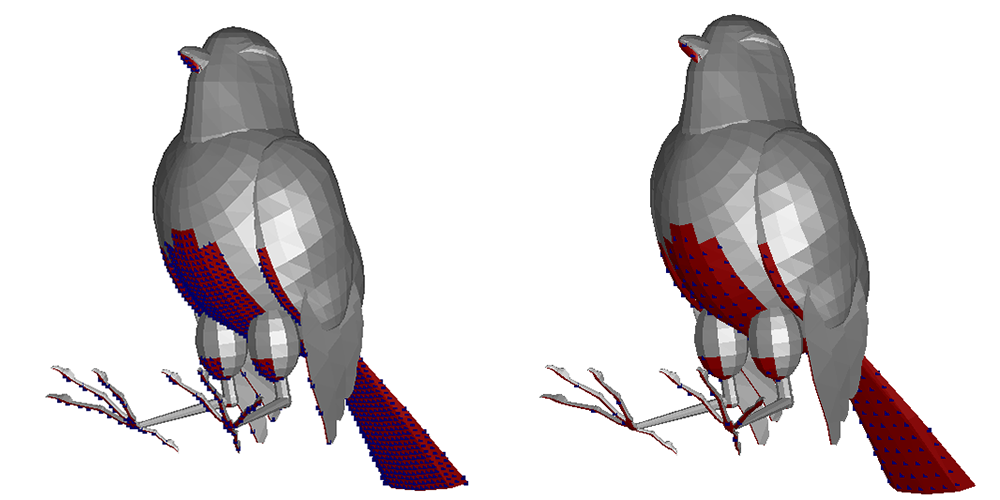
\includegraphics[width=1.0\textwidth]{Figure_3.png}
  	\caption{\textit{Result of different sampling distances. The left one uses 0.1mm as sampling distance while the right one uses 0.25mm.}}
	\end{figure}
	\subsection{Support Wireframe Generation}
	We defined the set of overhanging points to be $P$, the printing direction to be $\vec{v}$. To form the support structure, every point ${p}\in{P}$ should be connected to a point $s$. To ensure the printability of the support, the angle a between vector $\vec{s}p$ and $\vec{v}$ should be less than the critical angle $\alpha_{c}$. The valid points lie in a support cone $C$ from where the best $s$ point will be found for each ${p}\in{P}$. 
	\begin{figure}[!ht]
  		\centering
      	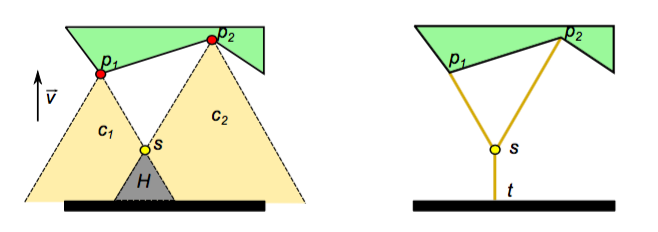
\includegraphics[width=0.8\textwidth]{Figure_4.png}
  	\caption{\textit{There are two overhang points $p_1$ and $p_2$ with supporting cones $C_1$ and $C_2$. We denote the intersection area of two cones and the ground as $H$ where the $s$ point for $p_1$ and $p_2$ lies.}}
	\end{figure}
	~\\~\\For the support tree, we define a geometric graph $G=(V,E)$ where V is the union of three kinds of points $V={P}\cup{S}\cup{T}$, where:
	\begin{itemize}
	\item P is a set of overhang points sampled on the mesh,
	\item S is a set of branching points connecting two parent points, and
	\item T is a set of points where the support intersects with model or the printing layer.
	\end{itemize}
	
	~\\The goal is to find the $T$ and $S$ in order to minimize the total length of the tree. This problem is related to the Euclidean Steiner Minimial Tree(ESMT) in 2D identified by HWang and Richard$\cite{tree}$, whose complexity is NP-complete. In this project, an ESMT is to be found in 3D space; thus the complexity is at least as NP-complete.$\cite{tree2}$ Therefore, in our implementation, we used a heuristic algorithm slightly different from that provided by the paper.$\cite{paper}$ This algorithm is based on greedy strategy. It finds local minimum for every point ${s}\in{S} and {s}\in{T}$ with minimum Euclidean Distance iteratively and find interseciton of two cones that leads to the sortest tree branch.

	\subsubsection{Method to obtain intersection of two cones}
	Given two overhanging points $p_1(x_1, y_1, z_1)$ and $p_2(x_2, y_2, z_2)$ with their corresponding cones $C_1$ and $C_2$ and critical angle $\alpha$. We can get a space $H$ for the candidate connection point $s$ (Figure 4) . We used a fast and simple method to obtain the best intersection point $s$.$\cite{cone1}$

	\begin{enumerate}
	\item Find the projection points of $p_1$ and $p_2$ on plane $y=0$$\cite{cone1}$. Denote them as $p_1^{'}$ and $p_2^{'}$.
	\item Calculate the Euclidean Distance $D=\sqrt{(p_1^{'}-p_2^{'})^{2}}$. 
	\begin{itemize}
	\item If $D\geq y_1\cot{(180-\alpha)}+y_2\cot{(\alpha)}$, $C_1$ and $C_2$ have no intersection. $p_1^{'}$ and $p_2^{'}$ are set to be the children of $p_1$ and $p_2$(intersection with ground). Stop.
	\item Else proceed step 3.
	\end{itemize}
	
	\item Find the plane $P$ where $p_1$, $p_2$, $p_1^{'}$ and $p_1^{'}$ lie in. Note that the plane p is perpendicular to the printing layer.
	\item Detect two lines $l_1$ and $l_2$. $l_1$ passes $_p1$ with slope $\tan{(180-\alpha)}$ on $P$ and $l_2$ passes $p_2$ with slope $\tan{(\alpha)}$.
	\item The intersection $s$ of $l_1$ and $l_2$ is the point connecting $p_1$ and $p_2$ with least distance.
	\end{enumerate}

	\subsubsection{Algorithm to build the tree}
	Given a list of overhang points $P$ and corresponding cones $C$, we used the algorithm 1 to form the tree structure.
	\begin{algorithm}
	\caption{Algorithm to build ESMT besed on greedy strategy}
	\SetKwInOut{Input}{Input}
	\SetKwInOut{Output}{Output}
	\Input{Overhang point list $P$ and corresponding Cone list $C$}
	\Output{Support point list $S$}
	define $D(p_i, p_j)=\sqrt{(p_i-p_j)^{2}}$ ~\\
	
	\While{$P$ is not empty}{
		\For{each ${p_i}\in{P}$}{
			find $p_j({i}\neq{j})$ where $D(p_i, p_j)=\min\limits_{j=1}^{|P|}D(p_i, p_j)$

			\eIf{$C_1$ and $C_2$ have no intersection}{
				set $p_i$ and $p_j$ as End Point
			}
			{
				denote intersecion as $s$~\\
				set $s$ to be child of $p_i$ and $p_j$
				add $s$ into $P$ as new overhang point
			}
			remove $p_i$ and $p_j$ from $P$~\\
			add $p_i$ and $p_j$ into $S$
		}	
	}
	~\\
	\For{each ${s_i}\in{S}$}{
		\If{$s_i$ is End Point}{
			\If{$s_i$ is not termial point}{
			set new point $s^{'}$ as the projection of $s_i$ on plane $y=0$~\\
			mark $s^{'}$ as termial point, set $s^{'}$ to be child of $s_i$~\\
			add $s^{'}$ into $S$
			}	
		}
		get child of $s_i$, denote as $s_c$~\\
		\If{segment($s_i$, $s_c$) has intersection with mesh}{
			find interseciton $s_c^{'}$ that minimize $D(s_i, s_c^{'})$~\\
			replace $s_c$ with $s_c^{'}$
		}
	}
	\end{algorithm}

	\begin{figure}[!ht]
  		\centering
      	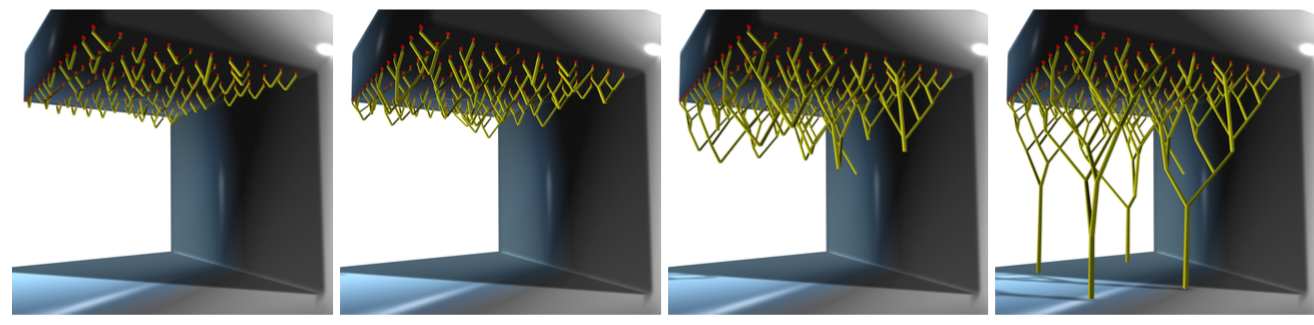
\includegraphics[width=\textwidth]{Figure_5.png}
  	\caption{\textit{The algorithm build structure progressively until all overhang points are support and the running time is reduced to $O(n^{2})$. The most expensive part is to detect the intersection of branches and mesh.}}
	\end{figure}
	~\\In the paper$\cite{paper}$, they used GPU and depth buffer to find the intersections. In our implementation, we simply applied brute force method to detect every branch intersection with the mesh, which led to one of the limitations.

	\subsection{Support Structure Design}
	In the paper, several structures are proposed for support. Only $N$ structure is accepted, because for one- and two-line structure, the support is not stable while for the closed profiles(circle, triangle and square), 3D printer tends to fill inside of them, leading to much more material used. $N$ structure can support the square area with relatively less material. According to the paper the diameter of the $N$ structure is determined by the formula: $d=k.l.\alpha$ where d is the struct diameter, $\alpha$ is the struct angle, and $k=0.0015$ from experiments. At the end of support structure, tips are added for easier removed form the model after printing.

	~\\In our implementation, besides the $N$ structure, we also implemented $X$ structure which is not mentioned in the paper but may lead to less material used. This structure has the stability for printing and also can support the square area.
	\begin{figure}[!ht]
  		\centering
      	
\includegraphics[width=0.6\textwidth]{Figure_6.png}
  	\caption{\textit{The N(left) and X(right) structure with increasing weight for each level.}}
	\end{figure}
	\begin{figure}[!ht]
  		\centering
      	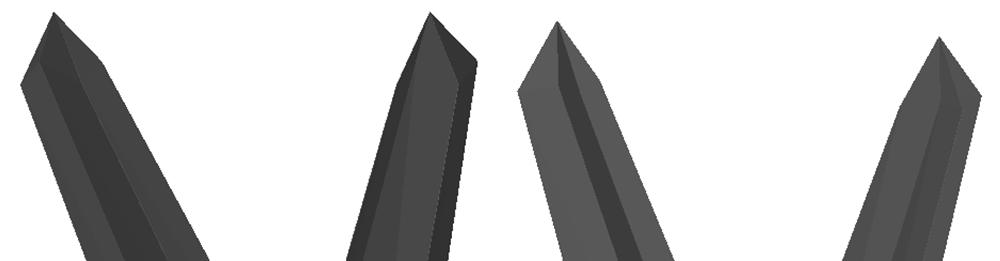
\includegraphics[width=0.6\textwidth]{Figure_7.png}
  	\caption{\textit{Tips structure added for N(left) and X(right) strucutre for easier removal of support material.}}
	\end{figure}
	\newpage

	\section{Summary}
	In this project, we implemented an optimization framework attempting to minimize the supporting structures needed for 3D printing objects with overhangs. The input is a 3D model represented by a manifold mesh. The model is first oriented in to a better position leading to less overhangs. Uniform sampling is applied to get the overhang points for the support structure which are also leaves of the support tree. Then the tree-like support structure is generated progressively using greedy strategy. At the end N/X structure is used to wrap the tree. And the output is obtained which is a rotated 3D model with support structure also composed of meshes. 
	~\\Appendix shows output of the program.
	~\\
	\subsection{Result and Evaluation}
	With some constraint, we were not able to print every model we implement with a 3D printer. Thus we used a self-defined evaluation method. The support structure will be composed of faces and vertices. And the amount of support material used is directly related to the area of the support faces, which can be calculated as $V=\sum\limits_{i=1}^{|F|}Area(F_i)$ where $F$ is the set of support faces. 

	~\\We performed evaluation based on the model with support provided by the author.
	\begin{table}[ht]
	\centering
	\label{my-label}
	\begin{tabular}{|l|l|l|l|l|l|l|}
		\hline
	Model      & Size  & Ref      & N Struct & Diff(N)   & X Struct  & Diff(X) \\
	\hline
	arches     & small & 9850.90  & 10197.90 & 3.52\%    & 9333.91   & -5.25\%  \\
	\hline
	armadillo  & small & 7001.35  & 6768.18  & -3.33\%    & 6196.41   & -11.50\% \\
	\hline
	bird       & small & 4463.55  & 4862.58  & 8.94\%    & 4903.30   & 9.85\%  \\
	\hline
	dragon     & large & 7274.38  & 4944.01  & -32.04\%   & 4575.10   & -37.11\% \\
	\hline
	mol\_thick & large & 9756.02  & 7602.45  & -22.07\%   & 7005.44   & -28.19\% \\
	\hline
	tree       & large & 14713.04 & 6834.60  & -53.55\%   & 6145.85   & -58.23\% \\
	\hline
	wheel      & large & 12551.00 & 17507.98 & 39.49\%   & 15948.13  & 27.07\% \\
	\hline
	\multicolumn{3}{|c|}{Average(all)} &\multicolumn{2}{|c|}{23.28\%} &\multicolumn{2}{|c|}{25.31\%}\\
	\hline
	\multicolumn{3}{|c|}{Average(small)} &\multicolumn{2}{|c|}{5.26\%} &\multicolumn{2}{|c|}{8.87\%}\\
	\hline
	\multicolumn{3}{|c|}{Average(large)} &\multicolumn{2}{|c|}{36.79\%} &\multicolumn{2}{|c|}{37.65\%}\\
	\hline
	\end{tabular}
	\caption{The amount of support material used in our implementation and the result provided by the author(Ref). The orientation is the same as the reference model by removing the support from the input file. Parameters: critical Angle $\alpha=50^{\circ}$, sampling distance $d=0.25mm$, thickness of material $t=0.1mm$. The difference is below 10\% for models with less details while larger for those with a lot more details. This is mainly caused by the difference in the algorithm applied to build the tree and the parameters setting from the author.}
	\end{table}
	\subsection{Limitation and Possible ways of improvement}
	\begin{enumerate}
	\item Cone-to-mesh intersection detection
	~\\We did not use the GPU and depth buffer to detect the intersection of support with mesh/printing layer. We instead used a brute force method and computed the intersection with whole mesh for every cone. This method is slow and expensive. To improve this, we can apply parallel computing on GPU, which computes the intersection of the cone with each face of the mesh in parallel.
	\item Support structure intersection with the model
	~\\We checked the intersection of cones with the mesh during building the support wireframe. If a branch of the tree is very closed to the mesh, it will not be detected to be intersected with the mesh. However, after wrapping the branches with N/X structure, there may be intersection between support and the mesh since each point on the branches is “expanded” to an area with diameter $d$. We did not detect the intersection because it`s very computationally expensive to detect intersection for every support face with the mesh. This may cause more material used and unprintability. To improve this, we may apply same method as in Cone-to-mesh intersection detection.
	\item Printability of the result in real case
	~\\The output of our implementation will be a rotated model with support structure. We did not check whether the support structure will be able to withstand the weight of mesh or shear forces during printing.$\cite{paper}$ We may first use some printing software for testing and then print the result using 3D printers.
	\item Global minimum not guaranteed
	~\\To generate the Euclidean Steiner Minimal Tree(ESMT), we used heuristic algorithm which leads to local minimum. Global minimum cannot be guaranteed because finding the ESMT with global minimum is NP-complete. Currently we cannot find out a way to improve this. 
	\end{enumerate} 
	We believe that most of the limitations could be addressed as future work of this project. Futhermore, besides having bi-furcation for the tree, we may have mutiple brahches which may save more support material.

	\newpage
	\addcontentsline{toc}{section}{References}
	\renewcommand\refname{References}
	\raggedright
	\bibliographystyle{unsrt}
	\bibliography{report}
	\newpage

	\addcontentsline{toc}{section}{Appendix}
	\begin{appendix}
	\begin{figure}[!ht]
  		\centering
      	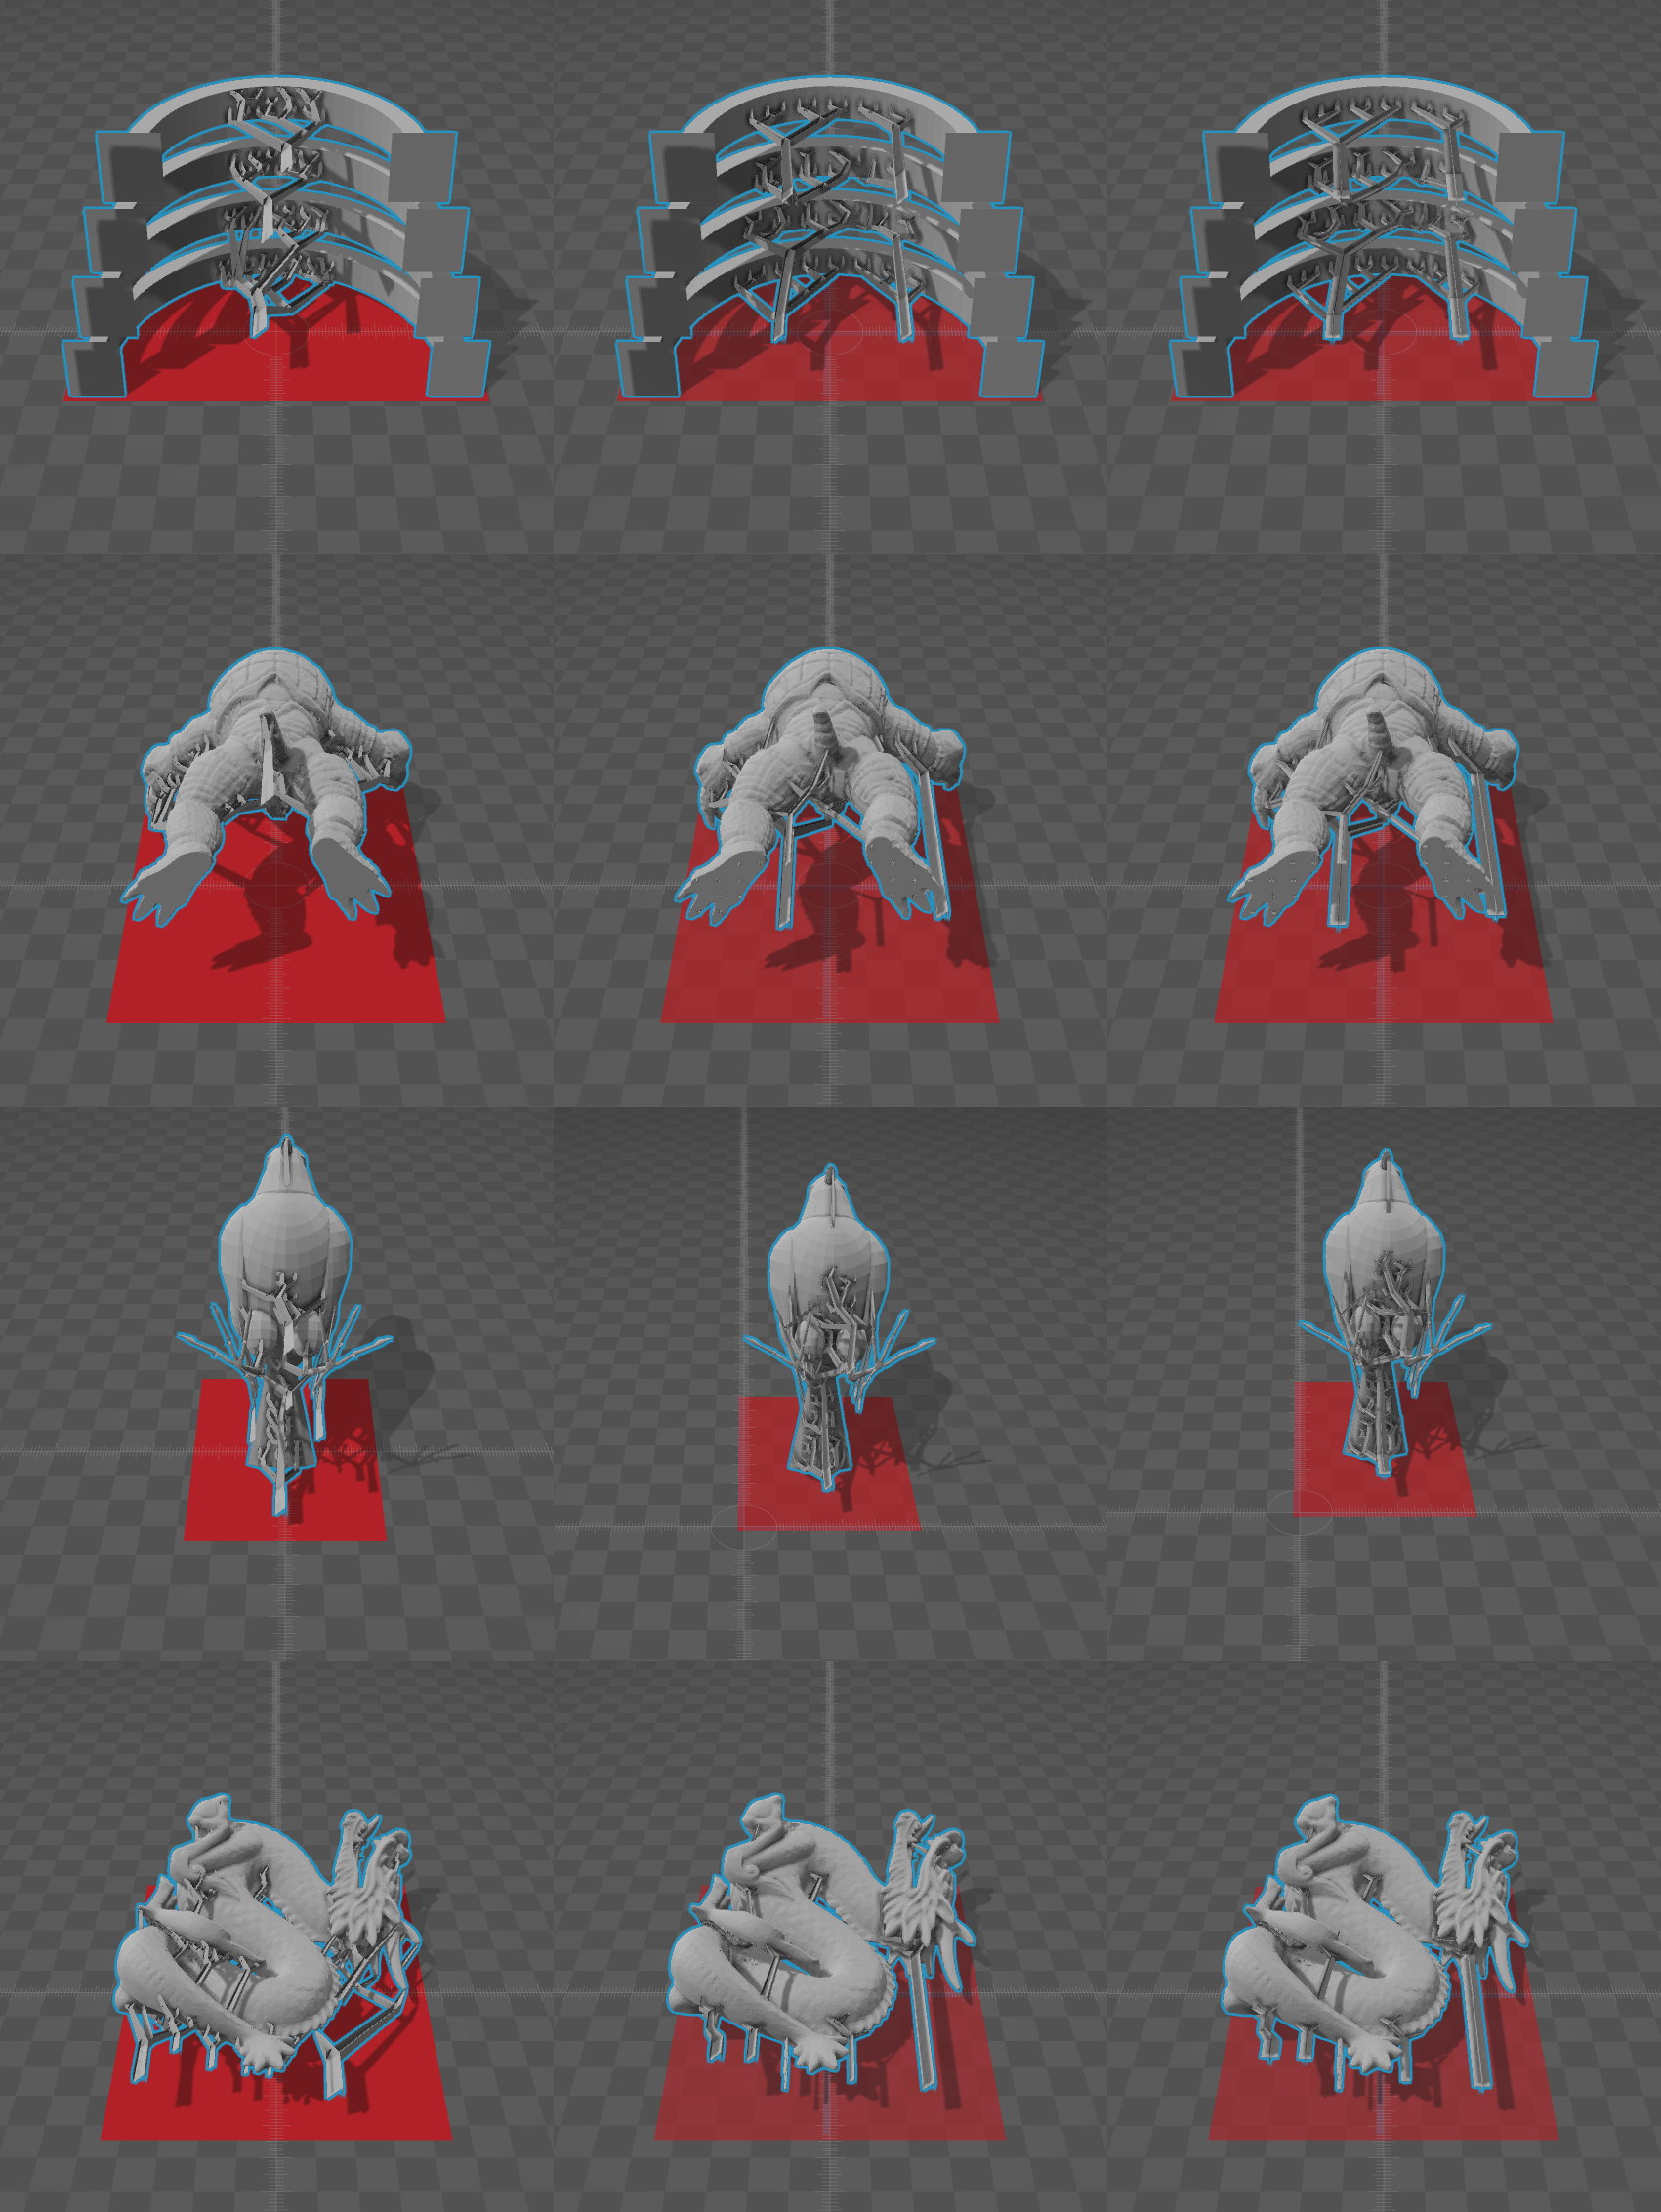
\includegraphics[width=\textwidth]{totalp1.png}
	\end{figure}
	\begin{figure}[!ht]
  		\centering
      	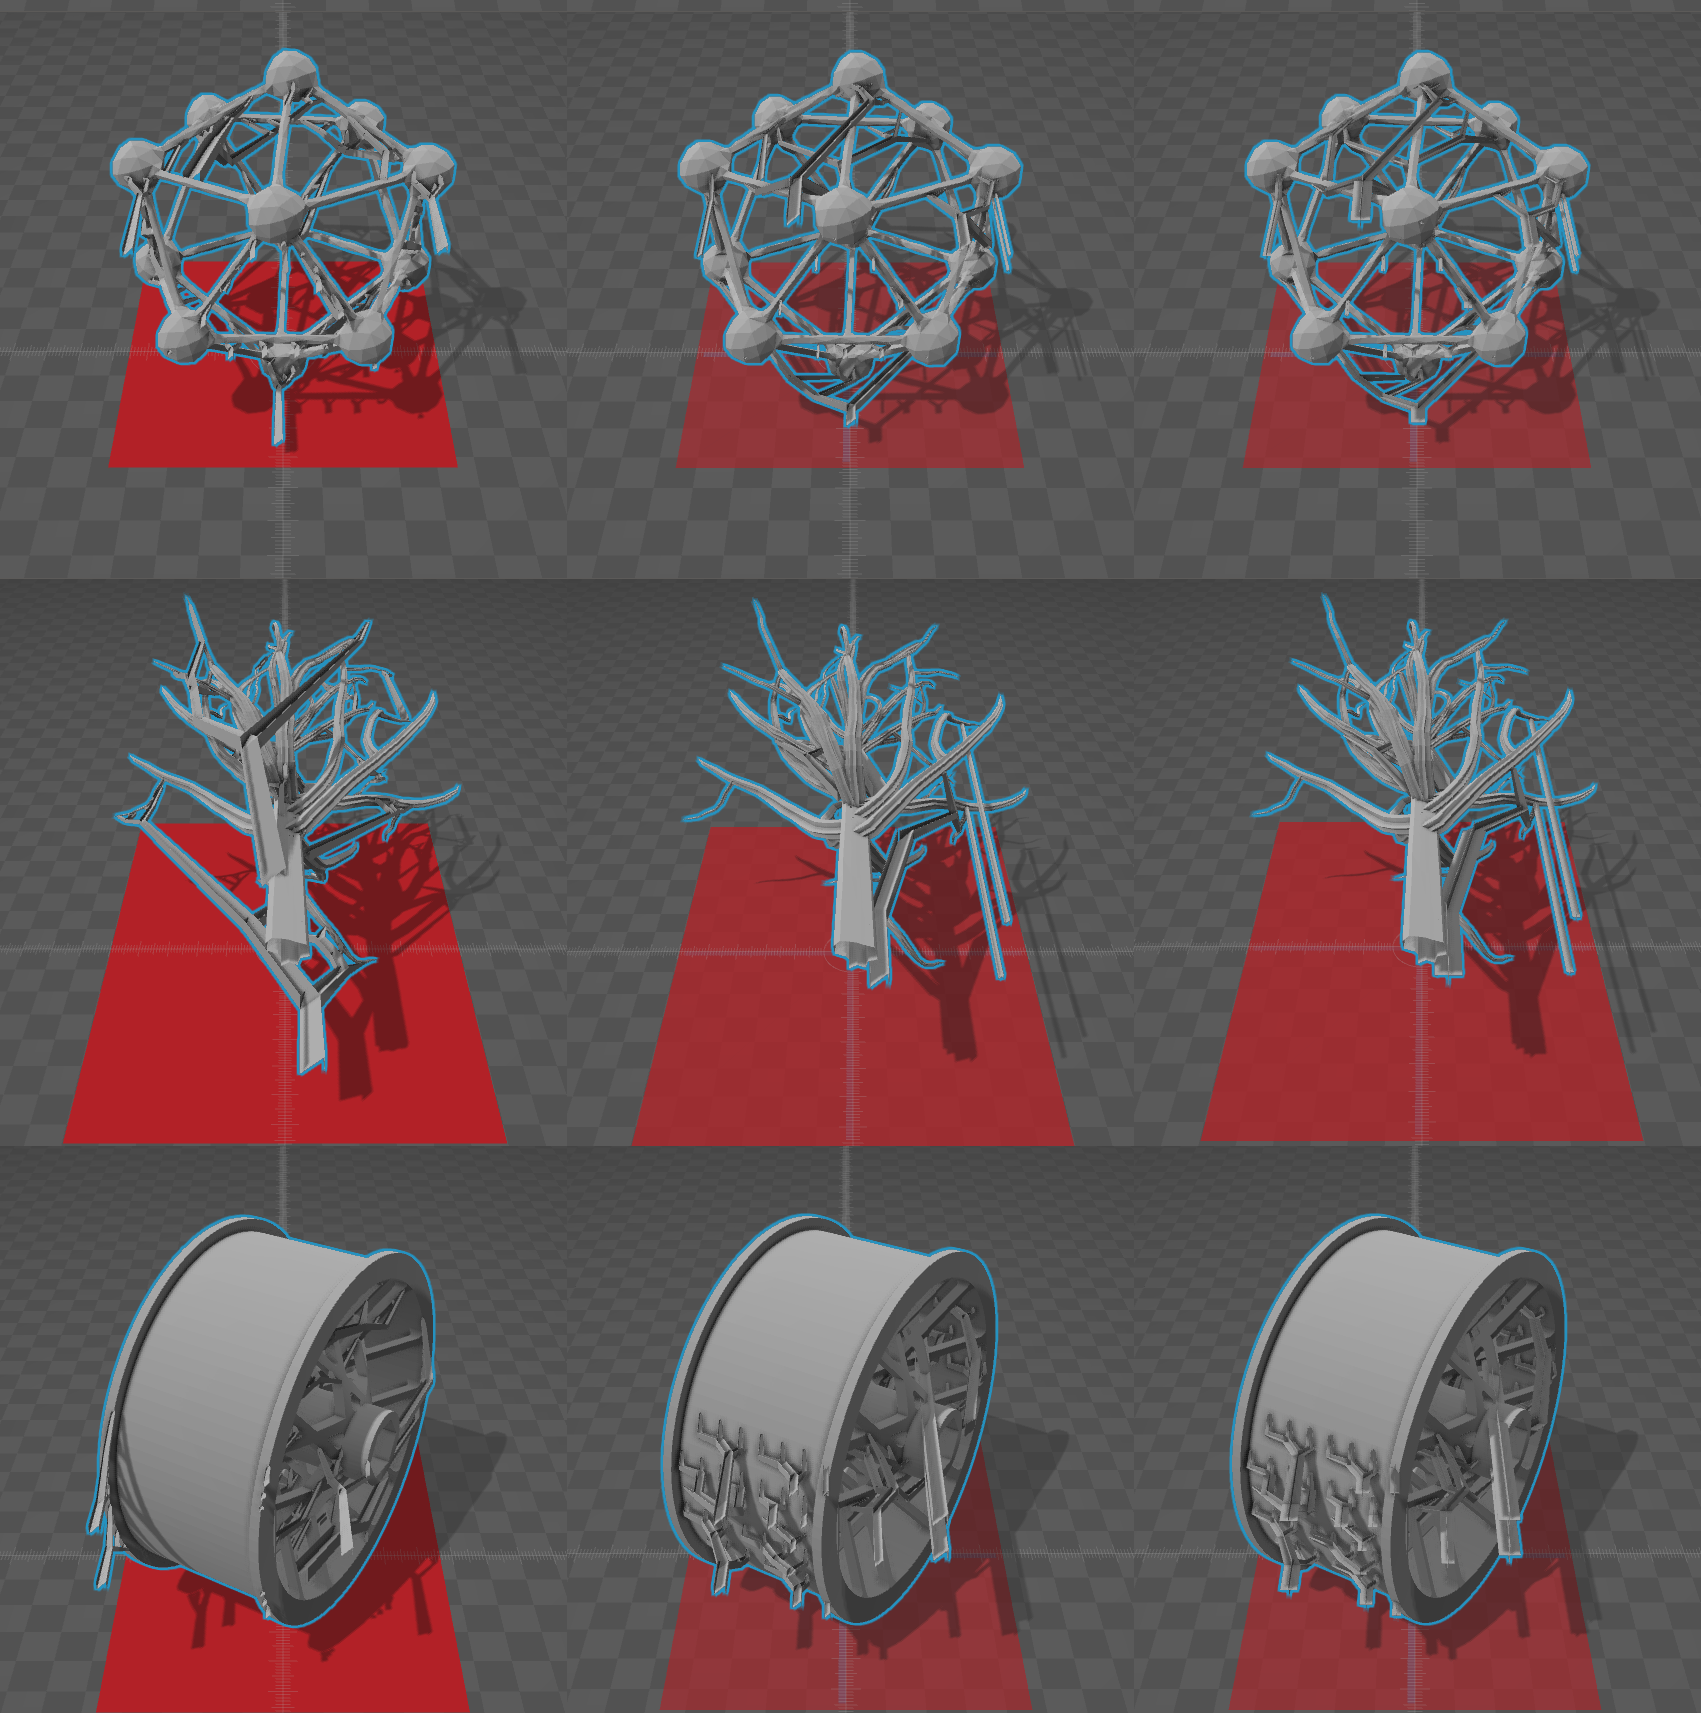
\includegraphics[width=\textwidth]{totalp2.png}
  	\caption{\textit{Left:Result provided by author, Mid:Our result with N structure, Right:Our result with X structure}}
	\end{figure}
	\end{appendix}
\end{document}


